% KSAS 2026 추계학술대회 포스터. A0 세로(841 x 1189 mm), 인쇄 규격 확정 2026-09-03.
% BUILD: python3 tools/render_poster.py
%   (numbers.tex를 만들고, make_poster_figures.py로 그림을 그린 뒤 xelatex를 두 번 돌린다)
% 결과 숫자는 하나도 손으로 적지 않는다. 전부 \NUM... 매크로이고, 출처는
% figures/paper1/occlusion_figure.json 이다. numbers.tex는 생성물이니 고치지 말 것.
% 판형은 엄격한 2단이다. 단을 가로지르는 요소는 머리글과 바닥글뿐이고, 본문과 그림은
% 모두 한 단 안에 들어간다. 가운데 세로줄은 tikz의 remember picture 로 그리므로
% xelatex 를 두 번 돌려야 자리를 잡는다.
% 빌드 로그의 "POSTER left/right height" 줄이 두 단의 높이(pt)다. 둘 중 큰 값이
% \textheight 에서 머리글과 바닥글을 뺀 값을 넘으면 두 쪽이 된다.
\documentclass[a0,portrait]{a0poster}
\usepackage[paperwidth=841mm,paperheight=1189mm,left=24mm,right=24mm,top=20mm,bottom=16mm]{geometry}

\usepackage{xetexko}
\setmainfont{NanumBarunGothic}
\setmainhangulfont{NanumBarunGothic}
\newfontfamily\latinfallback{lmsans10-regular.otf}   % NanumBarunGothic has no é
\usepackage{amsmath,amssymb}
\usepackage{graphicx}
\usepackage{booktabs}
\usepackage{xcolor}
\usepackage{array}
\usepackage{tikz}
\usetikzlibrary{calc}

\graphicspath{{./}{../../../figures/paper1/}}
\pagestyle{empty}
\setlength{\parindent}{0pt}
\setlength{\parskip}{3.0mm}
\renewcommand{\baselinestretch}{1.12}
\renewcommand{\arraystretch}{1.12}
\hyphenpenalty=10000
\setlength{\abovedisplayskip}{3mm}
\setlength{\belowdisplayskip}{3mm}

% one accent colour, slate text, grey rules: the palette of the figures
\definecolor{accent}{HTML}{2874A6}
\definecolor{slate}{HTML}{212F3D}
\definecolor{rulegrey}{HTML}{C8CED3}
\definecolor{mute}{HTML}{6B7783}
\color{slate}

\newcommand{\sect}[2]{\par\vspace{3.6mm}{\LARGE\bfseries\textcolor{accent}{#1}\hspace{6mm}#2\par}%
  \vspace{1mm}{\color{rulegrey}\rule{\linewidth}{1.4pt}}\par\vspace{2.5mm}}
\newcommand{\figcap}[2]{\par\vspace{1mm}{\small\textbf{#1}\ \ #2\par}}
\newcommand{\refnum}[1]{\textsuperscript{(#1)}}
\newcommand{\tabcap}[2]{{\small\textbf{#1}\ \ #2\par}\vspace{1.5mm}}
\newsavebox{\leftcol}\newsavebox{\rightcol}
\newlength{\colw}\setlength{\colw}{0.468\textwidth}

% GENERATED by tools/render_poster.py -- do not edit.
% source: figures/paper1/occlusion_figure.json (2026-08-31T16:58:56)

\newcommand{\NUMgenerated}{2026-08-31T16:58:56}
\newcommand{\NUMgit}{9f05cd5+dirty}
\newcommand{\NUMmachine}{Apple M2}
\newcommand{\NUMdegree}{8}
\newcommand{\NUMnseg}{48}
\newcommand{\NUMvmax}{5}
\newcommand{\NUMtimeweight}{40}
\newcommand{\NUMelastic}{10^{5}}
\newcommand{\NUMtrust}{1}
\newcommand{\NUMbaseArrival}{40.0}
\newcommand{\NUMbaseLos}{-2.17}
\newcommand{\NUMbaseLossLo}{14.96}
\newcommand{\NUMbaseLossHi}{16.52}
\newcommand{\NUMbaseLateral}{0.00}
\newcommand{\NUMbaseIters}{15}
\newcommand{\NUMbaseSolve}{0.19}
\newcommand{\NUMconArrival}{46.6}
\newcommand{\NUMconLos}{+3.34}
\newcommand{\NUMconLateral}{0.55}
\newcommand{\NUMconIters}{16}
\newcommand{\NUMconSolve}{0.46}
\newcommand{\NUMconClearance}{18.0}
\newcommand{\NUMgraft}{-1.69}
\newcommand{\NUMaxisBound}{43.0}
\newcommand{\NUMarrivalGap}{3.6}
\newcommand{\NUMsnapshot}{15.7}
\newcommand{\NUMdelay}{6.6}


\begin{document}

%======================================================================== header
\begin{minipage}[b]{0.62\textwidth}
{\veryHuge\bfseries 볼록 분해 없는 시공간 궤적 최적화\par}
\vspace{2mm}
{\Large\color{mute} 이동 장애물 회피와 가시선 유지\par}
\end{minipage}\hfill
\begin{minipage}[b]{0.36\textwidth}\raggedleft
{\Large 정현용\textsuperscript{*}, 이수원\quad{\large 국민대학교}\par}
\vspace{1.5mm}
{\large\color{mute} 한국항공우주학회 2026년도 추계학술대회, 하이원리조트, 2026-11-10\,--\,13\par}
\end{minipage}
\vspace{3mm}\par
{\color{accent}\rule{\textwidth}{2.4pt}}\par
\tikz[remember picture,overlay]\node[inner sep=0pt,outer sep=0pt] (coltop) {};

%======================================================================== left column
\sbox{\leftcol}{\begin{minipage}[t]{\colw}\raggedright

\sect{1}{임무 배경}
선회하는 비행체의 그림자가 회랑을 쓸고 지나가면, 회랑을 따라 비행하는 기체는 지상국과의 통신
링크를 잃는다.

도심항공교통(UAM) 기체는 지상국과 통신 링크를 유지하며 회랑을 비행한다. 다른 비행체가 지상국과
기체 사이에 들어오면 가시선이 가려지므로, 기체는 충돌뿐 아니라 그 비행체에 가려지는 영역, 곧
그림자도 피해야 한다. 둘 다 시간에 따라 움직이므로 경로와 통과 시점을 따로 정할 수 없다.

\begin{center}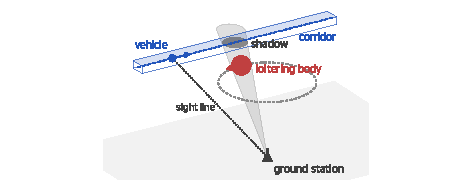
\includegraphics[width=0.32\linewidth]{concept_figure.pdf}\end{center}
\figcap{Fig.\ 1}{Mission scene (schematic): station, loitering body, its shadow on the corridor, and the sight line.}

\sect{2}{관련 연구}
기존 접근은 자유 공간을 볼록한 셀로 미리 분해하고, 어느 셀을 지날지를 볼록 완화로
고른다\refnum{1}. 리프팅은 이동 장애물을 정적인 집합으로 바꾸어 같은 분해를 등속 장애물까지
넓힌다\refnum{2}. 두 경우 모두 분해가 최적화 이전에 고정되므로, 장애물의 궤적이 휘거나 그림자처럼
회전하면 미리 만들어 둘 셀의 수가 늘어나고 통과 시각도 그 분해에 매인다.

본 논문은 분해도 시간 배분도 미리 정하지 않는다. 볼록 외부 근사를 순차 볼록 계획법(sequential
convex programming, SCP) 반복마다 현재 반복점 둘레의 구 위에 다시 세우므로, 관 전체가 볼록일
필요가 없다\refnum{3}.

\sect{3}{리프팅}
시간을 네 번째 좌표로 더해 리프팅하면 등속으로 움직이는 구형 keep-out zone(KOZ)은 기울어진
정적인 관, 곧 중심선 위의 각 점을 중심으로 하는 반지름 $r_m$의 구를 합친 집합이 된다. 결정
변수는 $N$차 곡선의 제어점 $Q_i=(x_i,\,t_i)$이고, De\,Casteljau 분할로 얻은 분할구간이 제약의
단위이다.

\begin{center}\includegraphics[width=0.58\linewidth]{fig_lift.pdf}\end{center}
\figcap{Fig.\ 2}{Lifting: a sphere at constant velocity becomes one static, tilted tube once time is a coordinate (1 s drawn as 1 m). 리프팅은 알려진 구성이다\refnum{2}. 본 논문은 이 관을 최적화 이전에 볼록 셀로 분해하지 않는다.}

\sect{4}{클리핑된 KOZ 볼륨}
분할구간의 제어점의 평균을 무게중심 $c$, $c$에서 그 제어점까지의 최대 거리를 $E$, $c$에서 KOZ
중심선까지의 거리를 $d$, 신뢰영역이 한 반복에서 제어점의 이동을 허용하는 최대 거리를 $\delta$라
하자. $c$를 중심으로 반지름 $r$의 구를 잡아 KOZ와의 교집합을 클리핑된 KOZ 볼륨 $L$로 정의한다.
\begin{equation}\tag{1}
r=\max\bigl(d,\ E+\delta\bigr)
\end{equation}
$d$가 $r_m+E+\delta$를 넘는 쌍은 닿을 수 없으므로 제약을 세우지 않는다. 하한 $E+\delta$는 다음
반복점의 분할구간을 구 안에 가두므로, $L$에 대한 반공간이 KOZ 전체에 대한 조건이 된다.

\begin{center}\includegraphics[width=0.58\linewidth]{fig_clip.pdf}\end{center}
\figcap{Fig.\ 3}{The clipped KOZ volume $L=\mathrm{KOZ}\cap B(c,r)$ around one segment of the trajectory, and the wall built on it.}

\sect{5}{근접 구간별 지지 반공간}
중심선 위의 점에서 $c$까지의 거리를 시간의 함수로 보고, 그 극대점마다 자른 조각이 근접
구간이다. 한 근접 구간에서 $c$에 가장 가까운 중심선의 점을 $p$, 법선을
$n=(c-p)/\lVert c-p\rVert$, 그 근접 구간이 만드는 클리핑된 KOZ 볼륨을 $L$, 분할구간의
제어점을 $Q_j$라 하면
\begin{equation}\tag{2}
b=\max\{\,n\cdot\xi:\ \xi\in L\,\},\qquad n\cdot Q_j\ \ge\ b
\end{equation}
$b$가 $L$의 지지값이므로 $L$은 반공간 밖에 남고, 같은 반공간을 모든 제어점에 부과하면 볼록
껍질 성질에 의해 분할구간 전체가 반공간 안에 놓인다. 관이 굽어 $c$를 감싸면 평면 하나로는
부족하지만, 극대점에서 자르면 근접 구간마다 반공간이 하나씩 생겨 그 사이의 틈이 허용 영역이 된다.
구와 반공간은 SCP 반복마다 다시 세운다.

\begin{center}\includegraphics[width=0.56\linewidth]{fig_halfspace.pdf}\end{center}
\figcap{Fig.\ 4}{A tube that wraps $c$: cut at the distance maximum ($\times$), one wall per approach segment, and the gap between the two walls is what they allow.}

\end{minipage}}

%======================================================================== right column
\sbox{\rightcol}{\begin{minipage}[t]{\colw}\raggedright

\sect{6}{볼록성 논의}
\begin{center}
\begin{tabular}{@{}p{0.29\linewidth}cp{0.52\linewidth}@{}}
\toprule
대상 & 볼록 & 의미 \\
\midrule
리프팅된 KOZ 관 & 아니오 & 전체에 대한 지지 반공간은 없다 \\
클리핑된 KOZ 볼륨 $L$ & 아니오 & 쓰는 것은 지지값 $b$ 하나이다 \\
분할구간 & 예 & 제어점의 볼록 껍질 안에 있다 \\
매 반복의 하위 문제 & 예 & 선형 부등식과 이차 목적함수 \\
\bottomrule
\end{tabular}
\end{center}
볼록 껍질 성질이 유한 개의 제어점에 대한 조건을 곡선 전체에 대한 조건으로 옮기며, 볼록성은
매 반복의 하위 문제에만 요구된다.

\sect{7}{최적화 문제}
\begin{equation}\tag{3}
\min\ \tfrac12\!\int_0^1\!\lVert x''(s)\rVert^2\,ds\ +\ w_t\,t_n
\end{equation}
\begin{equation}\tag{4}
t_{i+1}-t_i\ \ge\ \tau,\qquad \lVert x_{i+1}-x_i\rVert\ \le\ v_{\max}\,(t_{i+1}-t_i)
\end{equation}
식 (3)의 첫 항은 매끄러움 정규화 항, 둘째 항은 도착 시각 $t_n$의 선형 페널티 항이고, 식 (4)는
시간의 단조 증가와 제어 다각형의 변마다 부과하는 기울기 제한이다. 여기에 식 (2)와 회랑의 좌표
범위 제약을 함께 부과한다. 각 반복의 하위 문제는 식 (2)에 여유 변수를 두어 $w_s$를 곱해
목적함수에 더한 볼록 문제로, 신뢰영역 $\delta$ 안에서 푼다. 회피는 식 (2)의 제약이 담당하며,
목적함수에 장애물 페널티 항은 두지 않는다.

\sect{8}{가시선 차폐 제약}
지상국을 점광원으로 두면 장애물의 KOZ는 장애물 구와 그 뒤쪽 그림자를 합친 하나의 집합이다.
중심선이 드리우는 그림자는 곡면을 이루며, 이를 중심 곡면이라 한다. 4절과 5절의 구성을 중심선
대신 중심 곡면으로 그대로 적용한 것이 차폐 제약이다.

\sect{9}{실험 결과}
회랑 축은 그림자 중심이 회랑 고도에서 그리는 원에 접하므로, 그림자 점은 회랑을 따라 움직인다.
장애물 반지름 6\,m, 선회 반지름 30\,m, 고도 50\,m, 주기 80\,s, 회랑 200\,m, 고도
60--65\,m, 폭 $\pm$5\,m, 축 37.5\,m, $N=\NUMdegree$, 분할구간 \NUMnseg개,
$v_{\max}=\NUMvmax$\,m/s, $\tau=0.1$\,s, $w_t=\NUMtimeweight$, $w_s=\NUMelastic$,
$\delta=\NUMtrust$\,m, 도착 시각 자유.

\begin{center}\includegraphics[width=0.68\linewidth]{fig_scene.pdf}\end{center}
\figcap{Fig.\ 5}{The scenario in the lifted space: the corridor is a slab through time, the shadow spot's tube bends across it, and the two returned runs stay inside the corridor.}

\begin{center}
\tabcap{Table 1}{Results of the two runs.}
\begin{tabular}{@{}lrr@{}}
\toprule
 & 차폐 제약 없음 & 차폐 제약 부과 \\
\midrule
도착 시각 [s]            & \NUMbaseArrival & \NUMconArrival \\
최소 가시선 여유 [m]      & $\NUMbaseLos$   & $\NUMconLos$ \\
가시선 상실 구간 [s]      & \NUMbaseLossLo--\NUMbaseLossHi & 없음 \\
최대 횡방향 편차 [m]      & \NUMbaseLateral & \NUMconLateral \\
위반량 / 여유 변수        & 0 / 0 & 0 / 0 \\
반복 횟수 / 시간 [s]      & \NUMbaseIters\,/\,\NUMbaseSolve & \NUMconIters\,/\,\NUMconSolve \\
기준 시각 배분 시 여유 [m] & & $\NUMgraft$ \\
\bottomrule
\end{tabular}
\end{center}

기준 실행은 곧장 통과하여 그림자에 든 동안 가시선을 잃고, 차폐 제약을 부과한 실행은 같은 경로를
따르되 도착을 \NUMdelay\,s 늦춘다. 제약을 부과한 실행의 경로를 기준 실행의 시각 배분으로
비행하면 가시선 여유가 \NUMgraft\,m가 되어 가시선을 잃는다. 그림자만 피해 회랑 축을 따라 도달
가능한 시각의 하한은 \NUMaxisBound\,s이며, 차이 \NUMarrivalGap\,s는 리프팅된 KOZ의 시간 방향
두께가 낳는 보수성이다.

\begin{center}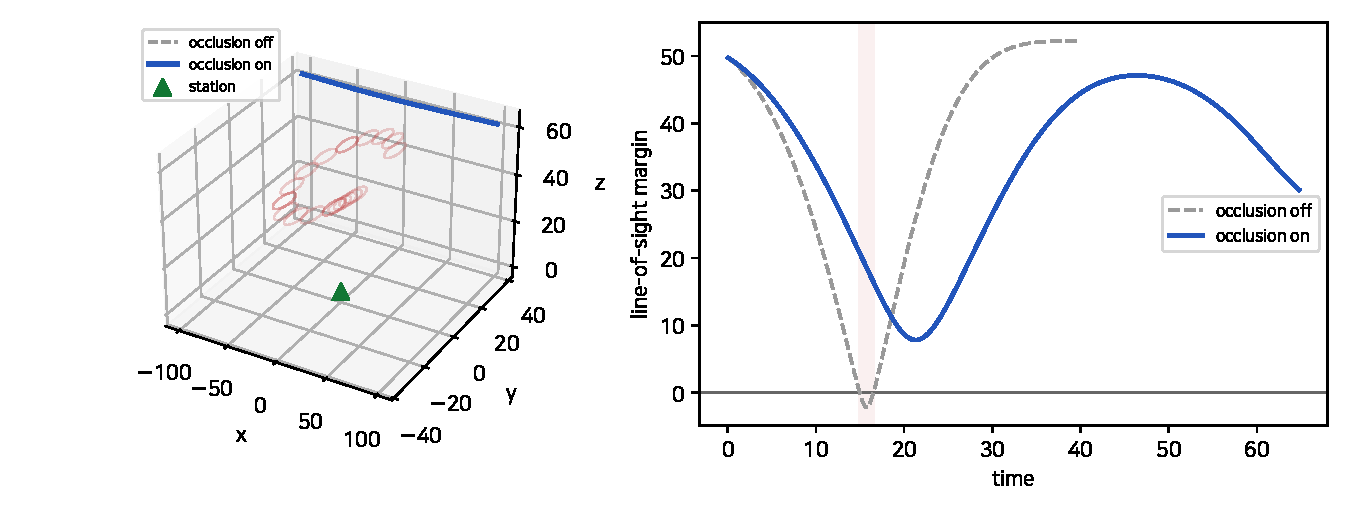
\includegraphics[width=0.70\linewidth]{occlusion_figure.pdf}\end{center}
\figcap{Fig.\ 6}{Scene at $t=\NUMsnapshot$\,s and sight margin against time.}

\sect{10}{결론 및 한계}
이동 장애물의 KOZ를 시공간의 관으로 두고, 무게중심 둘레의 구로 잘라낸 부분에 대한 지지 반공간을
SCP 반복마다 다시 세우는 정식화를 제시하였다. 볼록 분해와 시간 배분을 미리 정하지 않으므로,
관이 굽어 감싸는 경우에도 회피 조건은 근접 구간마다 반공간 하나로 표현되고 가시선 제약도 같은
구성으로 처리된다.

얻는 해는 초기값에 의존하는 국소해이며, 장애물의 운동은 알려져 있다고 가정한다. 시간 축 척도의
선택, 확률적 KOZ, receding horizon 구성을 향후 과제로 둔다.

\end{minipage}}
\typeout{POSTER left height \the\ht\leftcol\space + \the\dp\leftcol}
\typeout{POSTER right height \the\ht\rightcol\space + \the\dp\rightcol}
\typeout{POSTER textheight \the\textheight}
\noindent\usebox{\leftcol}\hfill\usebox{\rightcol}

\vfill
%======================================================================== footer
\tikz[remember picture,overlay]\node[inner sep=0pt,outer sep=0pt] (colbot) {};
{\color{rulegrey}\rule{\textwidth}{1.4pt}}\par
\vspace{1.5mm}
\begin{minipage}[t]{0.62\textwidth}
{\footnotesize\textbf{참고문헌}\par
(1) Marcucci, T., et al., ``Motion Planning around Obstacles with Convex Optimization,''
\textit{Science Robotics}, 8(84), 2023.\par
(2) Osburn, M. D., et al., ``Systematic Constraint Formulation and Collision-Free Trajectory
Planning Using Space-Time Graphs of Convex Sets,'' arXiv:2508.10203, 2025.\par
(3) Jeong, H.-Y., and Lee, S., ``Orbital Transfer Trajectory Design Method Using B{\latinfallback é}zier Curves,''
\textit{Proc.\ KSAS Fall Conference}, 2025.\par}
\end{minipage}\hfill
\begin{minipage}[t]{0.35\textwidth}
{\footnotesize\textbf{후기}\par
본 연구는 대한민국 정부(교육부)의 재원으로 한국연구재단의 4단계 BK21사업(2120240815267)의
지원을 받았음.\par
\vspace{1mm}
{\color{mute}Table 1, Fig.\ 5, Fig.\ 6의 모든 수치 출처: \texttt{figures/paper1/occlusion\_figure.json}
(\NUMgenerated,\ \NUMgit,\ \NUMmachine).}\par}
\end{minipage}

% the thin rule between the two columns, drawn between the two marks
\begin{tikzpicture}[remember picture,overlay]
  \coordinate (ctr) at ($(current page.west)!0.5!(current page.east)$);
  \draw[rulegrey,line width=1.1pt] ([yshift=-7mm]ctr |- coltop) -- ([yshift=7mm]ctr |- colbot);
\end{tikzpicture}

\end{document}
